
	\documentclass{article}
	\usepackage{amsmath,amssymb}
	\usepackage[inline]{enumitem}
	\usepackage{blindtext}
	\usepackage{booktabs}
	\usepackage{graphicx}
	\usepackage{xcolor}
	\usepackage[vmargin = 1.5in, top = 1in, bottom = 1.2in, letterpaper]{geometry}
	\usepackage{listings}
	\usepackage{courier}
	\usepackage{multicol}
	\usepackage{multirow}
	\usepackage{bm}
	\usepackage{algorithm}
	\usepackage{algpseudocode}
	\lstset{
	basicstyle = \small\tt,
	keywordstyle = \ttfamily\bfseries\color{blue},
	commentstyle = \it\color[cmyk]{1,0,1,0},
	stringstyle = \tt\color[RGB]{128,0,0},
	%frame = single,
	backgroundcolor = \color[RGB]{245,245,244},
	breaklines,
	extendedchars = false,
	xleftmargin = 2em,
	xrightmargin = 2em,
	aboveskip = 1em,
	tabsize = 4,
	showspaces = false
	showstringspaces = false
	}
	\begin{document}

	% \newfontfamily\courier{Courier New}


	\title{STAT 580 Homework 6}
	\author{Yifan Zhu}
	\maketitle

	\begin{enumerate}[leftmargin = 0 em, label = \arabic*., font = \bfseries]
	\item
	\begin{enumerate}
		\item 
		\begin{align*}
	\ell (\theta) & = \log \prod_{i=1}^n p(x_i - \theta)\\
	& = \sum_{i=1}^n \log p(x_i - \theta)\\
	& = \sum_{i=1}^n \left( - \log \pi - \log(1 + (x_i - \theta)^2) \right)\\
	& =  -n \log \pi - \sum_{i=1}^{n} \log \left( 1 + (\theta - x_i)^2 \right) 
	\end{align*}

	\begin{align*}
	l'(\theta) & = - \sum_{i=1}^n \frac{1}{1 + (x_i - \theta)^2} \cdot 2 (\theta - x_i)\\
	& = - 2 \sum_{i=1}^n \frac{\theta - x_i}{1 + (\theta - x_i)^2}
	\end{align*}

	\begin{align*}
	l''(\theta) & = -2 \sum_{i=1}^n \frac{\left( 1 + (\theta - x_i)^2 \right) - 2 (\theta - x_i)^2 }{\left( 1 + (\theta - x_i)^2 \right)^2 }\\
	& = -2 \sum_{i=1}^n \frac{1 - (\theta - x_i)^2}{\left(1 + (\theta - x_i)^2\right)^2}
	\end{align*}
	\item 
	\begin{align*}
	I(\theta) & = - E_\theta (l''(\theta))\\
	& = n \int_{-\infty}^\infty \frac{(p'(x))^2}{p(x)} \mathrm{d}x\\
	& = n \int_{-\infty}^\infty \frac{4 x^2}{\pi (1 + x^2)^3} \mathrm{d}x\\
	& = 2n \int_0^\infty \frac{4 x^2}{\pi (1 + x^2)^3} \mathrm{d}x \\
	& = 2 n \frac{x (x^2 - 1) + (x^2 + 1) \arctan x}{2 \pi (x^2 + 1)^2} \bigg|_{0}^\infty\\
	& = 2 n \frac{\pi/2}{2 \pi} \\
	& = \frac{n}{2}
	\end{align*}

	\item \ 

	\lstinputlisting[language = R]{./Codes/p1c.R}

	\begin{center}
		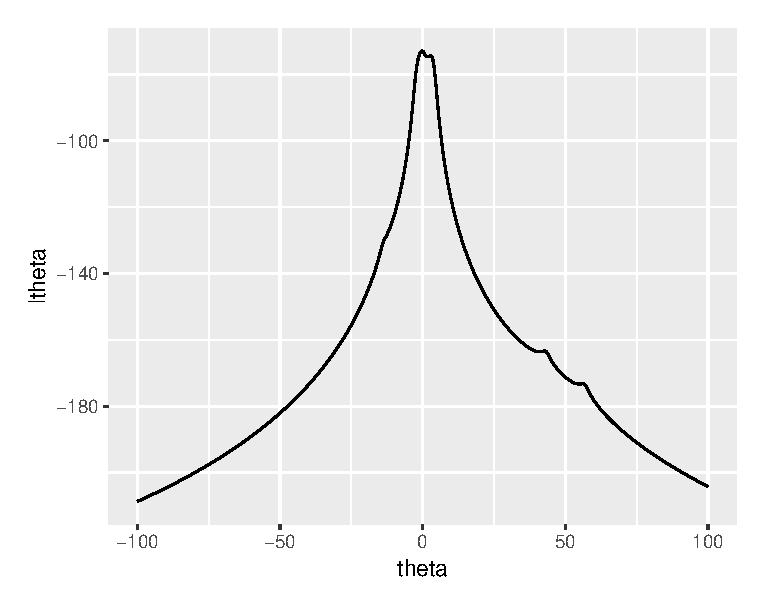
\includegraphics[width = 0.7\textwidth]{ltheta.eps}
	\end{center}

	\item \ 

	\lstinputlisting[language = R]{./Codes/p1d.R}

	Results:

		\begin{tabular}{*{5}{c}}
		\toprule
		-11& -1& 0& 1.4& 4.1\\
		\midrule
		 Not Converge & -0.1922865 & -0.1922865 & 1.713569 & 2.817473 \\
		 \bottomrule
		\end{tabular}

		\begin{tabular}{*{4}{c}}
		\toprule
		4.8& 7& 8& 38 \\
		\midrule
		Not Converge & 41.04099 & Not Converge & 42.79593\\
		\bottomrule
		\end{tabular}

	\item 
	Results:

		\begin{tabular}{*{5}{c}}
		\toprule
		-11& -1& 0& 1.4& 4.1\\
		\midrule
		 -0.1922866 & -0.1922866 & -0.1922866 & -0.1922866 &  2.817474 \\
		 \bottomrule
		\end{tabular}

		\begin{tabular}{*{4}{c}}
		\toprule
		4.8& 7& 8& 38 \\
		\midrule
		 2.817474 &  2.817474 & 2.817474 & 2.817474\\
		\bottomrule
		\end{tabular}

		In this way the algorithm is more stable. We do nat have non-convergence case and the results is not sensitive about the starting points.


	
	\end{enumerate}

	\item 
	\begin{enumerate}
		\item \ 
		\lstinputlisting[language = R]{./Codes/p2a.R}

		Then we have 
		\[\hat{\theta}_1 = \frac{1}{\hat{\beta}_0} = 1/103.49 = 0.00966,\, \hat{\theta}_2 = \frac{\hat{\beta}_1}{\hat{\beta}_0} = 110.42 / 103.49 = 1.066963\]

		\item 
		\begin{align*}
		g(\bm \theta) & = - \sum_{i=1}^n \left( y_i - \frac{\theta_1 x_i}{x_i + \theta_2} \right)^2\\
		\frac{\partial^2 g}{\partial \theta_1} &= 2 \sum_{i=1}^n \left( y_i - \frac{\theta_1 x_i}{x_i + \theta_2} \right) \frac{x_i}{x_i + \theta_2}\\
		\frac{\partial g}{\partial \theta_2} &= -2 \sum_{i=1}^n \left( y_i - \frac{\theta_1 x_i}{x_i + \theta_2} \right) \frac{\theta_1 x_i}{(x_i + \theta_2)^2} \\
		\frac{\partial^2 g}{\partial \theta_1^2} & = -2 \sum_{i=1}^n \frac{x_i^2}{(x_i + \theta_2)^2}\\
		\frac{\partial^2 g}{\partial \theta_2^2} & = 2 \sum_{i=1}^n \left( \frac{2 \theta_1 x_i y_i}{(x_i + \theta_2)^3} - \frac{3 \theta_1^2 x_i^2}{(x_i + \theta_2)^4} \right)\\
		\frac{\partial^2 g}{\partial \theta_1 \partial \theta_2} &= 2 \sum_{i=1}^n \left( \frac{2 \theta_1 x_q^2}{(x_i + \theta_2)^3} - \frac{x_i y_i}{(x_i + \theta_2)^2} \right)  
		\end{align*}

		Then 
		\[\bm \theta_{t+1} = \bm \theta_{t} - \left(\frac{\partial^2 g}{\partial \bm \theta \partial \bm \theta^T}\right)^{-1} \frac{\partial g}{\partial \bm \theta}\bigg|_{\bm \theta = \bm \theta_t}\]

		Codes:

		\lstinputlisting[language = R]{./Codes/p2b.R}
		
		\item \ 

		\lstinputlisting[language = R]{./Codes/p2c.R}

		\item 
		\begin{align*}
		f_i (\bm \theta) & = \frac{\theta_1 x_i}{x_i + \theta_2}\\
		\frac{\partial f_i}{\partial \theta_1} & = \frac{x_i}{x_i + \theta_2}\\
		\frac{\partial f_i}{\partial \theta_2} & = - \frac{\theta_1 x_i}{(x_i + \theta_2)^2}
		\end{align*}

		\lstinputlisting[language = R]{./Codes/p2d.R}
		


	\end{enumerate}
	
 	\end{enumerate}

	\end{document}
